\documentclass[11pt]{article}
\usepackage[margin=1in]{geometry}
\usepackage{amsmath,amssymb}
\usepackage{booktabs}
\usepackage{graphicx}
\usepackage{caption}
\usepackage{float}
\usepackage{natbib}
\usepackage{setspace}
\usepackage[hidelinks]{hyperref}
\linespread{1.08}
\setlength{\parskip}{0.35em}
\graphicspath{{figures/}}
\captionsetup{font=small,labelfont=bf}

\title{\textbf{State-versus-County Aggregation and Identification in U.S.\ Monetary
Policy Transmission to Employment, 2002--2019}}
\author{Abdallah Dalis\\ \small DePaul University, Department of Economics\\ \small ECO 508: Predictive Analytics and Time Series Analysis}
\date{June 2026}

\begin{document}
\maketitle

\begin{abstract}
\noindent A shift-share (Bartik) difference-in-differences design applied to U.S.\ county
employment returns a \emph{positive} response to federal-funds-rate tightening---the opposite
of the contractionary effect predicted by theory and recovered by textbook vector
autoregressions. This paper asks whether that reversal reflects spatial aggregation or
\emph{identification}. Using a county employment panel (2002--2019), Bauer--Swanson
high-frequency monetary policy surprises, and FRED macro series, I estimate four time-series
models: a reduced-form VAR, a recursively identified structural VAR, Jord\`a local projections,
and a random forest. The reduced-form and structural VARs both deliver the conventional
negative employment response on a pre-ZLB sample (trough $\approx -0.38\%$), while the same
VAR estimated over 2002--2019 inverts because the zero lower bound renders the funds rate an
uninformative policy indicator. Replacing the endogenous rate change with the identified
high-frequency surprise in the shift-share design \emph{flips the exposure interaction from a
significant positive ($+0.20$ to $+1.25$) to negative ($-0.39$ to $-2.42$) across horizons}---
evidence pointing to identification, rather than aggregation, as the driver, though the
surprise-based estimates are imprecise. The random forest lowers RMSE relative to na\"ive benchmarks but has
zero correlation with realized employment growth, indicating variance shrinkage rather than
genuine predictability. The central methodological lesson: endogeneity of the policy instrument
can manufacture a sign reversal in an otherwise standard regional design.
\end{abstract}

\clearpage

\section{Introduction}

A long tradition in regional macroeconomics holds that contractionary monetary policy reduces
employment, and that interest-sensitive local economies---those concentrated in construction
and durable manufacturing---contract \emph{more} \citep{carlino1998}. A shift-share
difference-in-differences (DiD) design I estimated in prior work reverses this prediction:
interacting the quarterly change in the federal funds rate with predetermined 2002
construction-plus-manufacturing exposure across $\sim$2{,}900 U.S.\ counties yields a
\emph{positive, statistically significant} coefficient ($+0.0202$, s.e.\ $0.0045$;
cumulative four-quarter effect $+0.042$). Read literally, high-exposure counties \emph{gain}
employment when the Fed tightens---a result at odds with both theory and the conventional
vector-autoregression (VAR) evidence.

This paper asks a precise question: \textbf{is the positive sign an artifact of spatial
aggregation, or of identification?} The two explanations have very different implications.
If aggregation drives it, the county design is measuring something real that disappears at
coarser geographies. If identification drives it, the problem is that the realized funds-rate
change is endogenous---it rises precisely when the economy (and interest-sensitive sectors)
is booming---so the ``effect'' is reverse causation, and replacing the endogenous rate with an
exogenous monetary \emph{shock} should restore the contractionary sign.

The gap I address is that regional transmission studies rarely confront the two explanations
head-on within a single, internally consistent research design. I do so by holding the
shift-share structure fixed and varying only the source of policy variation, while
benchmarking against national VAR/SVAR systems and a machine-learning forecaster. Concretely,
I estimate four of the methods on the ECO~508 list: a reduced-form \textbf{VAR}, a recursively
identified \textbf{SVAR}, Jord\`a \textbf{local projections} (LP) using Bauer--Swanson
high-frequency surprises as the identified shock, and a \textbf{random forest} (RF) for
employment-growth forecasting. The full-panel DiD is retained only as motivating evidence, not
re-estimated as a headline result.

Three findings emerge. First, the reduced-form and structural VARs deliver the textbook
negative employment response on a pre-ZLB sample (cumulative trough $\approx -0.38\%$), but the
\emph{same} specification estimated over 2002--2019 inverts to a positive response---because
the zero-lower-bound (ZLB) episode of 2008--2015 pins the funds rate near zero and destroys its
content as a policy measure. Second, and centrally, when I replace the endogenous rate change
with the identified surprise inside the shift-share design, the exposure interaction
\emph{flips sign} from significantly positive to negative at every horizon, though the
surprise-based estimates are not individually significant given limited high-frequency
variation. Third, the random forest attains lower out-of-sample RMSE than na\"ive benchmarks but
has essentially zero correlation with realized employment growth, a cautionary illustration of
variance shrinkage masquerading as skill. The remainder of the paper reviews the relevant
literature (\S2), describes the data (\S3) and methodology (\S4), presents results (\S5), and
concludes (\S6).

\section{Literature Review with Paper Summaries}

The empirical benchmark for this paper is \citet{carlino1998}, who ask whether U.S.\ regions
respond differently to a common monetary policy shock and whether structural features explain the
heterogeneity. They estimate a structural VAR in output, prices, and the funds rate across eight
BEA regions over 1958--1992, tracing regional personal-income responses to a funds-rate innovation.
A core of regions tracks the national average, but the durable-manufacturing-heavy Great Lakes
contracts more sharply while the Rocky Mountains and Southwest contract less, with the gaps lining
up with industry mix and small-firm shares. Theirs is the canonical statement of the prediction my
difference-in-differences design violates: greater interest-sensitivity should mean a \emph{larger}
contraction, not an employment gain, so a positive county response signals that identification,
rather than a genuine regional regularity, is at work.

\citet{coibion2012} asks why the estimated size of monetary effects is so method-sensitive,
reconciling the small effects implied by recursive VARs with the large effects implied by the
Romer--Romer narrative approach. Working with postwar U.S.\ aggregates, he shows that once the
contractionary impetus, the reserves-targeting period, and lag length are accounted for, the real
effects are consistent across schemes and ``medium''-sized. The relevance for my project is
twofold: it legitimizes placing VAR and local-projection responses on a common scale, and it warns
that sample period and lag choice can swing conclusions---a warning that proves central to my
zero-lower-bound result.

On identification, \citet{cee1999} supply the template for my structural VAR. They ask what the
dynamic effects of a monetary shock are and how sensitive those effects are to identifying
assumptions, using recursive (Cholesky) identification on U.S.\ aggregates with the funds rate
ordered after slow-moving output and prices. A contractionary shock produces a hump-shaped decline
in output and employment that peaks after one to two years, alongside the familiar ``price
puzzle.'' That timing restriction and the expected hump-shaped contraction are exactly what my
benchmark SVAR reproduces.

My primary estimation vehicle is the local projection of \citet{jorda2005}, motivated by the goal
of estimating impulse responses without committing to a full dynamic system. The method regresses
the outcome at each horizon directly on the shock---one regression per horizon---with
heteroskedasticity- and autocorrelation-consistent standard errors. Jord\`a shows these responses
are robust to dynamic misspecification and nest VAR responses as a special case, at some cost in
efficiency. This is what lets me trace the county employment response to an external monetary shock
horizon by horizon rather than imposing a panel VAR.

\citet{plagborg2021} then ask whether that choice of estimator matters, proving that local
projections and VARs estimate the same population impulse responses given comparable lag
structures. The result is theoretical, with finite-sample simulations showing the two differ only
through a bias--variance trade-off. For my paper this means any divergence between the LP and the
VAR/SVAR reflects finite-sample and shock-measurement differences, not the estimator---so the
LP-versus-VAR comparison can be read as a consistency check rather than a contest.

The shock that feeds those projections comes from the high-frequency identification literature.
\citet{gss2005} ask whether asset-price responses to FOMC announcements can isolate unanticipated
policy, using thirty-minute changes in money-market futures around announcements. They find that
two factors are needed---a current-rate surprise and a path surprise---establishing that
narrow-window futures changes capture the component of policy markets did not expect. This is the
methodological foundation for treating a high-frequency surprise as an exogenous shock.

\citet{nakamura2018} use such surprises to measure monetary non-neutrality and to test for a
``Fed information effect,'' studying real-rate and expectations responses in thirty-minute windows
around announcements. They find sizable real effects but also that surprises move expected output
growth in a direction suggesting announcements reveal the central bank's private read on the
economy. Their information effect is the leading alternative explanation for perverse-signed
responses, which I carry explicitly into my limitations.

\citet{bauerswanson2023}, whose orthogonalized monthly surprise series I adopt, ask whether
high-frequency surprises are truly exogenous given evidence they are predictable. Using an expanded
announcement sample, they show raw surprises are partly forecastable from pre-announcement
macro-financial conditions and recommend orthogonalizing them. I use their cleaned series, and I
document that it is essentially uncorrelated with the \emph{realized} quarterly funds-rate
change---the reason an instrumental-variables projection is infeasible here and the surprise must
enter directly as the shock.

\citet{gertlerkaradi2015} formalize how such surprises identify structural responses as external
instruments, asking what monetary policy does to activity and credit costs in a proxy-SVAR
instrumented by funds-futures surprises. They find that modest movements in short rates generate
large movements in credit spreads alongside a textbook output contraction, while
\citet{stockwatson2018} give the general conditions under which this external-instrument approach
(equivalently, LP--IV) is valid. This is the design I first attempt, abandoning the
instrumental-variables version only once its quarterly first stage proves degenerate.

\citet{jarocinski2020} push the information-effect concern furthest, asking whether surprises can
be decomposed into pure monetary and central-bank information shocks. Within a structural VAR they
use the sign of the co-movement between interest rates and stock prices around announcements to
separate the two: pure tightenings produce textbook contractions, information shocks produce
opposite-signed responses, and conventional surprises blend them. This is the sharpest alternative
reading of my puzzle---an exposure design built on contaminated surprises could itself generate a
perverse positive response---so I flag it as the most important unresolved threat.

Because my design is itself a shift-share (Bartik) object, its identification deserves equal
scrutiny. \citet{gpss2020} ask precisely what a shift-share instrument identifies, showing
analytically that it is numerically equivalent to using the predetermined exposure shares as
instruments. Identification therefore rests on the exogeneity of the shares and is driven largely
by the cross-section. This disciplines how I read the exposure interaction and points to the
shares---and the endogeneity of the shock interacted with them---as the threat to identification.

\citet{borusyak2022} develop the complementary view, asking when identification can instead rest
on the \emph{shocks}. They show shift-share IV is valid under many quasi-randomly assigned shocks,
provided no small set of shocks dominates. Both warnings bite in my setting: with few and
endogenous monetary ``shifts'' and exposure shares plausibly correlated with county
characteristics, a shift-share design is exactly the configuration in which an endogenous policy
rate can flip a coefficient's sign.

The machine-learning component is motivated by \citet{medeiros2021}, who ask whether
machine-learning methods improve macroeconomic forecasting in a data-rich environment. Using a
large U.S.\ macro dataset and rolling out-of-sample evaluation, they find random forests outperform
factor and autoregressive benchmarks for inflation, owing to data-driven variable selection and
nonlinearity. I adopt their lagged-feature, rolling-window protocol; my own finding---that the
forest lowers RMSE for employment growth yet carries no directional skill---serves as a
counterpoint about when such methods genuinely help.

Taken together, the applied regional work fixes the benchmark prediction---contractionary policy
lowers employment, more so where interest-sensitivity is high---while the identification and
shift-share literatures explain how that prediction can appear to reverse in practice. Every method
I use is disciplined by this body of work: the structural VAR follows \citet{cee1999}, the
projections follow \citet{jorda2005} under the equivalence established by \citet{plagborg2021}, the
shock follows \citet{bauerswanson2023} within the high-frequency tradition of \citet{gss2005} and
\citet{nakamura2018}, and the cross-sectional design is read through \citet{gpss2020} and
\citet{borusyak2022}. The contribution of this paper is to hold that cross-sectional design fixed
and vary only the source of policy variation, isolating whether the puzzling positive sign reflects
spatial aggregation or identification, while recognizing that the information-effect decomposition
of \citet{jarocinski2020} and shadow-rate measures such as \citet{wuxia2016} mark the natural next
steps.

\section{Data}

County employment is the third-month establishment employment
level from the QCEW (Quarterly Census of Employment and Wages), 2002Q1--2019Q4, for $\sim$2{,}889
counties; the log level is the outcome. Predetermined exposure is the 2002 county share of
employment in construction and durable manufacturing, built from County Business Patterns (CBP),
treated as time-invariant (the shift-share ``shares''). National macro series are from FRED:
the effective federal funds rate (\texttt{FEDFUNDS}), total nonfarm payrolls (\texttt{PAYEMS}),
and the CPI (\texttt{CPIAUCSL}), all monthly. The identified monetary shock is the
\citet{bauerswanson2023} orthogonalized high-frequency surprise (monthly, summed to quarters for
the panel; San Francisco Fed update, covering 1988--2023). Employment and prices enter as
$100\times\Delta\log$; the funds rate enters in levels and first differences.

The county panel and surprise series are aligned at
quarterly frequency over 2002--2019 (72 quarters). The national VAR/SVAR use monthly data; the
benchmark VAR is estimated on 1976--2008 (a clean, pre-ZLB modern sample) and re-estimated on
2002--2019 to isolate the ZLB's effect. Table~\ref{tab:summary} reports summary statistics.
Employment growth and inflation are mildly left-skewed and leptokurtic, reflecting the 2008--09
collapse; the funds-rate change is sharply non-normal (excess kurtosis $15.9$) because it is
near-zero throughout the ZLB and moves only in discrete tightening/easing episodes.

\begin{table}[H]\centering
\caption{Summary statistics, 2002--2019 (monthly)}\label{tab:summary}
\small
\begin{tabular}{lrrrrrr}
\toprule
Series & Mean & Std.\ dev. & Min & Max & Skew. & Kurt. \\
\midrule
Fed funds rate (level, \%) & 1.420 & 1.581 & 0.07 & 5.26 & 1.226 & 0.424 \\
$\Delta$ Fed funds rate & $-0.001$ & 0.141 & $-0.96$ & 0.25 & $-3.001$ & 15.883 \\
Employment growth ($\Delta\log\times100$) & 0.068 & 0.158 & $-0.62$ & 0.40 & $-1.998$ & 5.194 \\
Inflation ($\Delta\log$ CPI$\times100$) & 0.175 & 0.295 & $-1.786$ & 1.367 & $-1.430$ & 10.310 \\
\bottomrule
\end{tabular}
\end{table}

Figure~\ref{fig:series} plots the three
national series with the ZLB window (Dec 2008--Dec 2015) shaded. The funds rate falls to the
ZLB in late 2008 and stays there through 2015, so $\Delta$FFR is essentially zero for seven
years while employment recovers steadily---the mechanical source of the positive
employment-to-tightening comovement documented below. Table~\ref{tab:adfkpss} reports augmented
Dickey--Fuller (ADF) and KPSS tests. Inflation is clearly stationary on both tests. For the
funds-rate change and employment growth the picture is the familiar mixed one: the ADF cannot
reject a unit root at the data-driven lag (a reflection of its low power on short, persistent
series) while KPSS is borderline, and monthly payroll growth carries enough residual seasonality
to nudge its KPSS statistic past the 5\% line. The funds-rate \emph{level} is non-stationary
(ADF $p=0.46$; KPSS rejects), as expected for a near-integrated policy rate. Following standard
practice, all VAR/SVAR variables therefore enter in stationary ($\Delta\log$ or first-differenced)
form.

\begin{table}[H]\centering
\caption{Stationarity tests (2002--2019)}\label{tab:adfkpss}
\small
\begin{tabular}{lcc}
\toprule
Series & ADF $p$-value & KPSS $p$-value \\
\midrule
Fed funds rate (level) & 0.464 & 0.010 \\
$\Delta$ Fed funds rate & 0.263 & 0.100 \\
Employment growth & 0.454 & 0.018 \\
Inflation & 0.010 & 0.100 \\
\bottomrule
\end{tabular}
\\[2pt]
\footnotesize ADF $H_0$: unit root. KPSS $H_0$: stationarity.
\end{table}

\begin{figure}[H]\centering
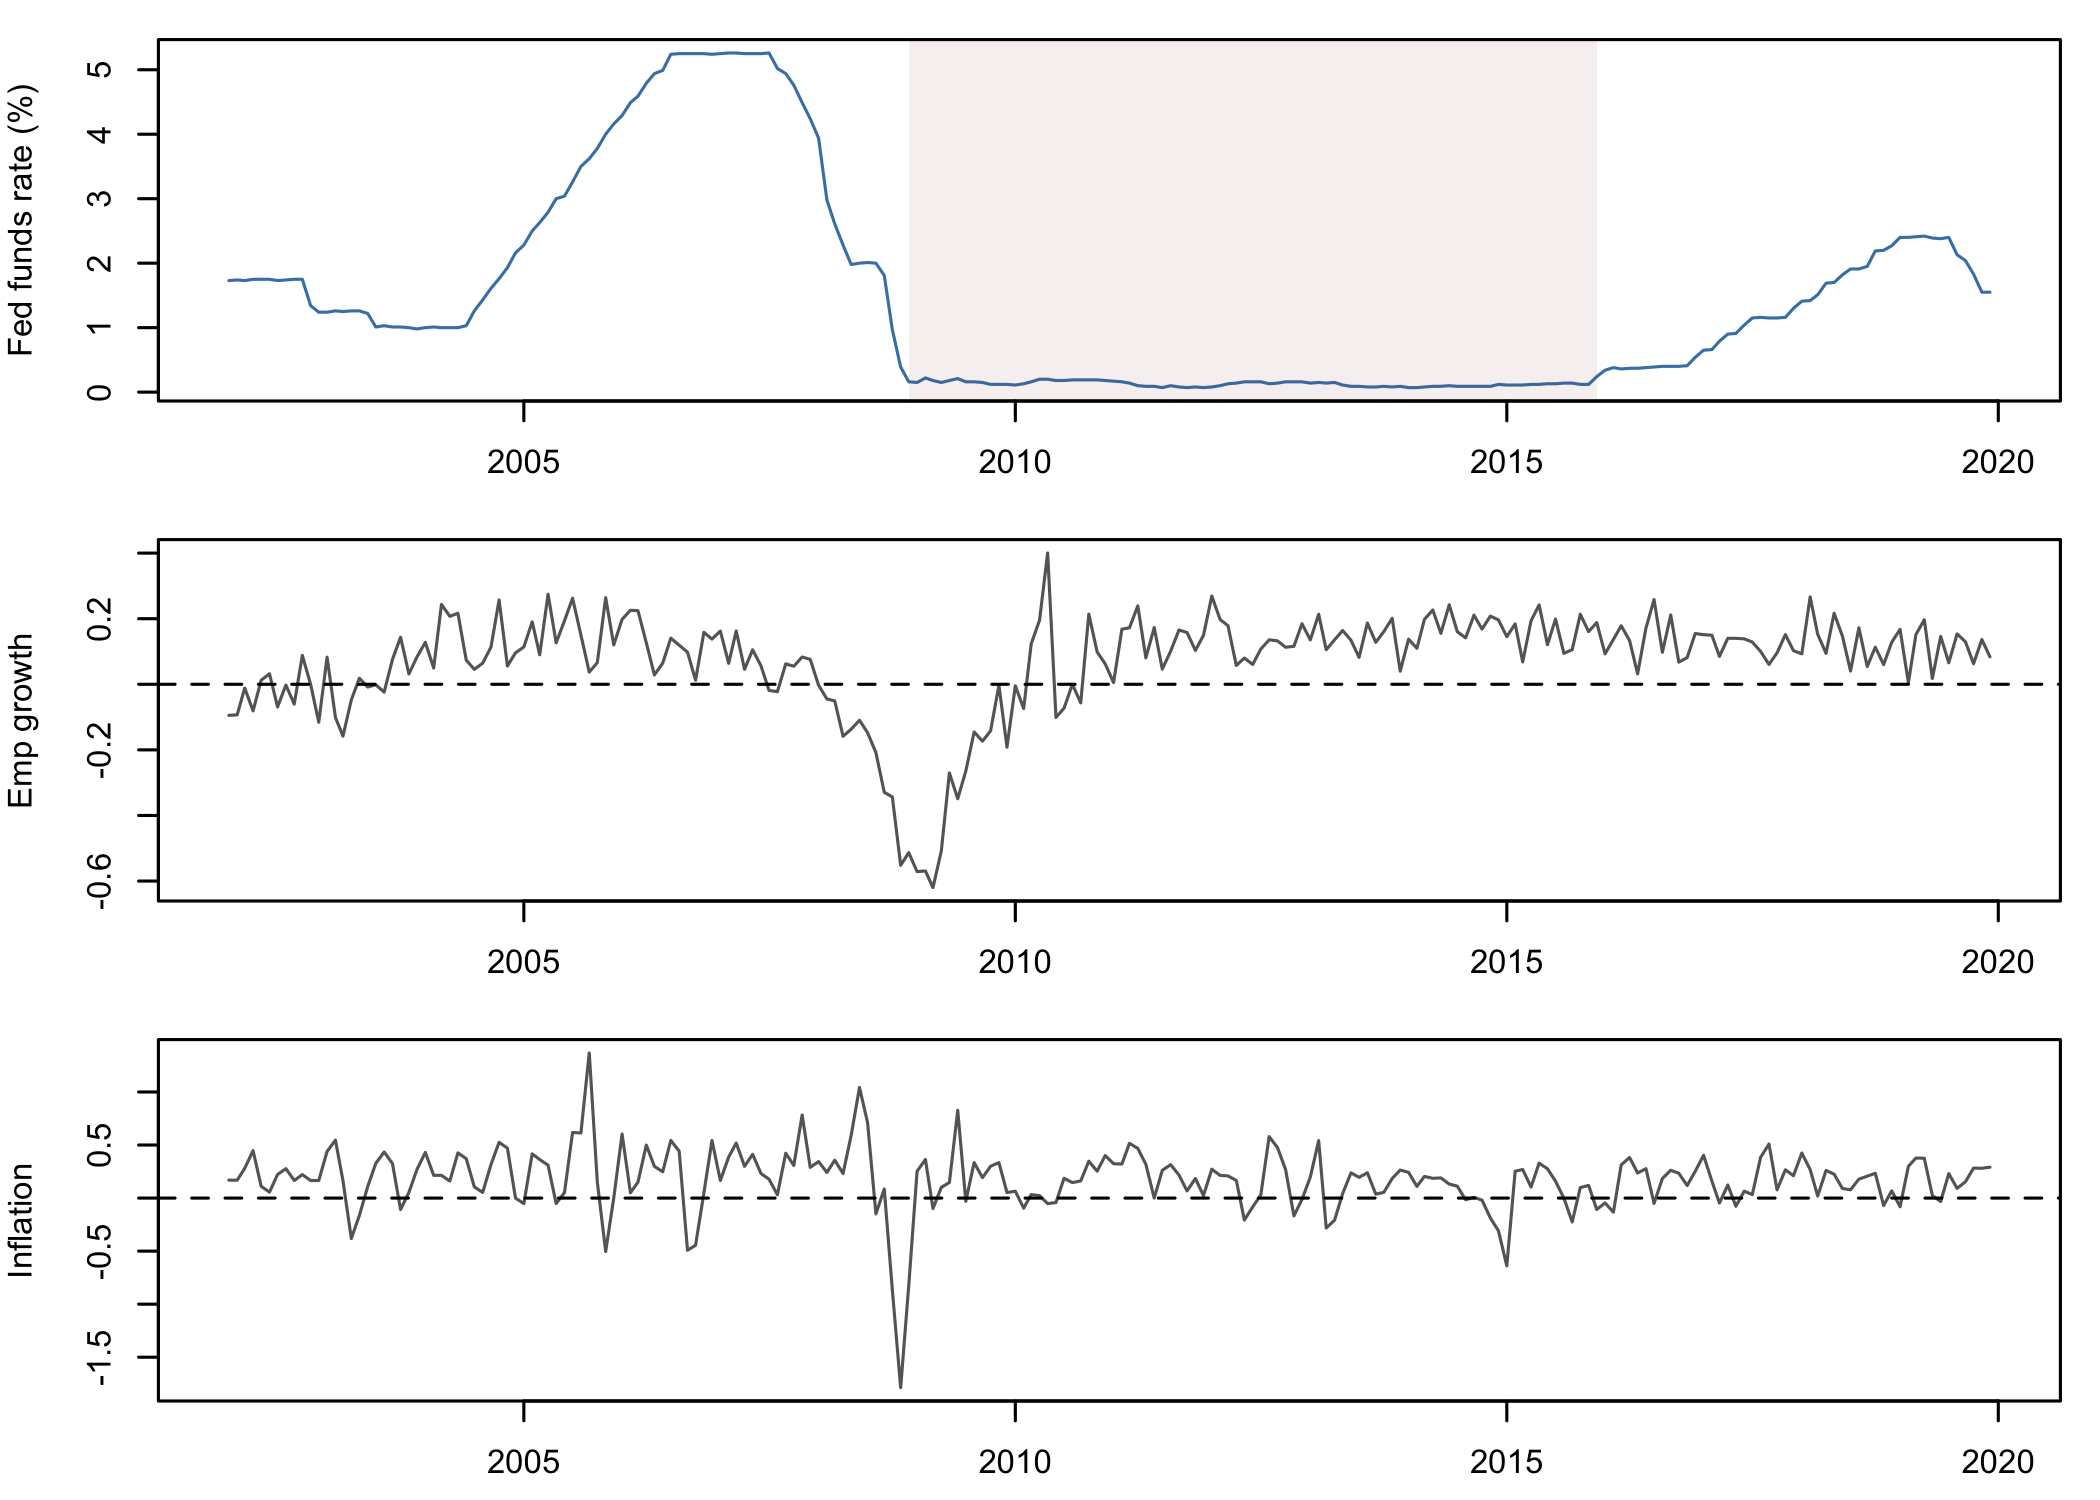
\includegraphics[width=0.82\textwidth]{fig1_series.png}
\caption{U.S.\ monetary and labor-market series, 2002--2019. Shaded band marks the zero-lower-
bound episode (Dec 2008--Dec 2015), during which $\Delta$FFR is pinned near zero.}
\label{fig:series}
\end{figure}

\section{Empirical Methodology}

The analysis applies four of the methods on the ECO~508 list, each chosen to serve a distinct
role in adjudicating the puzzle. Throughout, let $\pi_t=100\,\Delta\log\text{CPI}_t$ denote
monthly inflation, $n_t=100\,\Delta\log\text{PAYEMS}_t$ employment growth, and $r_t$ the federal
funds rate with $\Delta r_t$ its change.

The national benchmark is a reduced-form vector autoregression in $y_t=(\pi_t,n_t,\Delta r_t)'$,
\begin{equation}
y_t = c + \sum_{k=1}^{p} A_k\, y_{t-k} + u_t, \qquad u_t\sim(0,\Sigma_u),
\end{equation}
with the lag length $p$ chosen by the AIC, SC, and HQ criteria; from it I report Granger-causality
tests, forecast-error variance decompositions, and impulse responses with bootstrap confidence
bands. To give the policy innovation an economic interpretation, I identify a structural monetary
shock recursively in the manner of \citet{cee1999}, writing $u_t=B\varepsilon_t$ with $B$ the
lower-triangular Cholesky factor of $\Sigma_u$ and the funds rate ordered last,
\begin{equation}
\begin{pmatrix} u^{\pi}_t \\ u^{n}_t \\ u^{r}_t \end{pmatrix}
=\begin{pmatrix} b_{11} & 0 & 0 \\ b_{21} & b_{22} & 0 \\ b_{31} & b_{32} & b_{33}\end{pmatrix}
\begin{pmatrix} \varepsilon^{\pi}_t \\ \varepsilon^{n}_t \\ \varepsilon^{\text{MP}}_t \end{pmatrix}.
\end{equation}
Equation~(2) is the identifying restriction matrix: the zero restrictions encode the assumption
that prices and employment do not respond to the monetary shock $\varepsilon^{\text{MP}}_t$
within the month, while the policy rate may respond to all contemporaneous information. The three
structural innovations are a price (supply) shock $\varepsilon^{\pi}_t$, a real-activity
(employment) shock $\varepsilon^{n}_t$, and the monetary policy shock $\varepsilon^{\text{MP}}_t$,
with the recursive ordering letting each affect the variables ordered after it contemporaneously.

The cross-sectional design rests on local projections. For the focused panel of major counties
$i$, the \citet{jorda2005} specification regresses the cumulative change in log employment $\ell$
on the identified shock at each horizon $h$,
\begin{equation}
100\big(\ell_{i,t+h}-\ell_{i,t-1}\big)=\alpha_i^{h}+\delta_t^{h}+\beta_h\, s_t + \text{controls} + \epsilon_{i,t+h},
\end{equation}
where $s_t$ is the Bauer--Swanson orthogonalized surprise entered directly as the shock. The
central identification test adds the exposure interaction,
\begin{equation}
100\big(\ell_{i,t+h}-\ell_{i,t-1}\big)=\alpha_i^{h}+\delta_t^{h}+\theta_h\,\big(\text{shock}_t\times \widetilde{\text{exp}}_i\big)+\epsilon_{i,t+h},
\label{eq:lpint}
\end{equation}
and is estimated twice: once with $\text{shock}_t=\Delta r_t$, the endogenous funds-rate change
that drives the difference-in-differences puzzle, and once with $\text{shock}_t=s_t$, the
identified surprise, where $\widetilde{\text{exp}}_i$ is standardized exposure. County and time
fixed effects absorb the level of the shock and of exposure, so $\theta_h$ is identified purely
from the differential response by exposure; I cluster standard errors by quarter, since the
identifying variation lives in the seventy-two quarterly shocks (clustering by quarter is the
panel analog of a Newey--West HAC correction, absorbing the within-quarter cross-sectional
dependence a pure time-series HAC would miss). I use the surprise as a direct
shock rather than as an instrument for $\Delta r_t$ because the quarterly first stage is empty:
regressing $\Delta r_t$ on the orthogonalized surprise yields $F\approx0$ ($R^2\approx0$). Since the orthogonalized surprise does not move the
realized rate, the external-instrument approach of \citet{gertlerkaradi2015} and
\citet{stockwatson2018} is infeasible here, and using the surprise directly is the standard
fallback \citep{coibion2012}.

The fourth method is a random forest that forecasts employment growth $n_t$ from a matrix of
twelve lags each of $n$, $\pi$, and $\Delta r$---thirty-six predictors, all lagged so that no
contemporaneous information enters and look-ahead bias is ruled out by construction. I evaluate it
out of sample on a rolling, expanding-window basis, refitting each year and benchmarking against a
random walk and a seasonal-naive (twelve-month) forecast using RMSE, MAE, and directional accuracy. The evaluation logic is consistent across methods: the VAR and SVAR
are judged by the shape of their impulse responses and variance decompositions, the local
projections by the horizon-$h$ response and the sign of $\theta_h$, and the random forest by its
rolling out-of-sample loss against the na\"ive benchmarks. All estimation is carried out in the
accompanying R script, which reproduces every table and figure end-to-end.

\section{Results}

\subsection{Reduced-form VAR}
Lag-selection criteria disagree (Table~\ref{tab:varlag}): AIC and FPE choose $p=12$, SC and HQ
choose $p=3$; I report the AIC system. On the 1976--2008 benchmark, $\Delta$FFR Granger-causes
employment ($p=0.003$; Table~\ref{tab:granger}), and the funds rate accounts for $\sim$6.5\% of
the employment forecast-error variance at two years (Table~\ref{tab:fevd}). The cumulative
employment response to a contractionary shock is negative and hump-shaped, with a trough near
$-0.38\%$ (Figure~\ref{fig:varirf}, left). Re-estimating the identical specification on
2002--2019 \emph{inverts} the response to strongly positive ($+2.45\%$ at $h=12$;
Figure~\ref{fig:varirf}, right): with the funds rate pinned at the ZLB for seven years,
$\Delta$FFR carries almost no policy content and the VAR recovers reverse causation (rates rise
as employment recovers).

\begin{table}[H]\centering
\begin{minipage}[t]{0.32\textwidth}\centering
\caption{VAR lag selection}\label{tab:varlag}\small
\begin{tabular}{lc}\toprule Criterion & Lag \\ \midrule AIC & 12 \\ SC (BIC) & 3 \\ HQ & 3 \\ FPE & 12 \\ \bottomrule\end{tabular}
\end{minipage}\hfill
\begin{minipage}[t]{0.32\textwidth}\centering
\caption{Granger causality}\label{tab:granger}\small
\begin{tabular}{lc}\toprule Null & $p$ \\ \midrule $\Delta$FFR $\nrightarrow$ emp. & 0.003 \\ emp. $\nrightarrow$ $\Delta$FFR & $<0.001$ \\ \bottomrule\end{tabular}
\end{minipage}\hfill
\begin{minipage}[t]{0.32\textwidth}\centering
\caption{FEVD of employment}\label{tab:fevd}\small
\begin{tabular}{lccc}\toprule & $\pi$ & $n$ & $\Delta r$ \\ \midrule $h{=}6$ & .03 & .93 & .04 \\ $h{=}12$ & .03 & .90 & .07 \\ $h{=}24$ & .08 & .86 & .07 \\ \bottomrule\end{tabular}
\end{minipage}
\end{table}

\begin{figure}[H]\centering
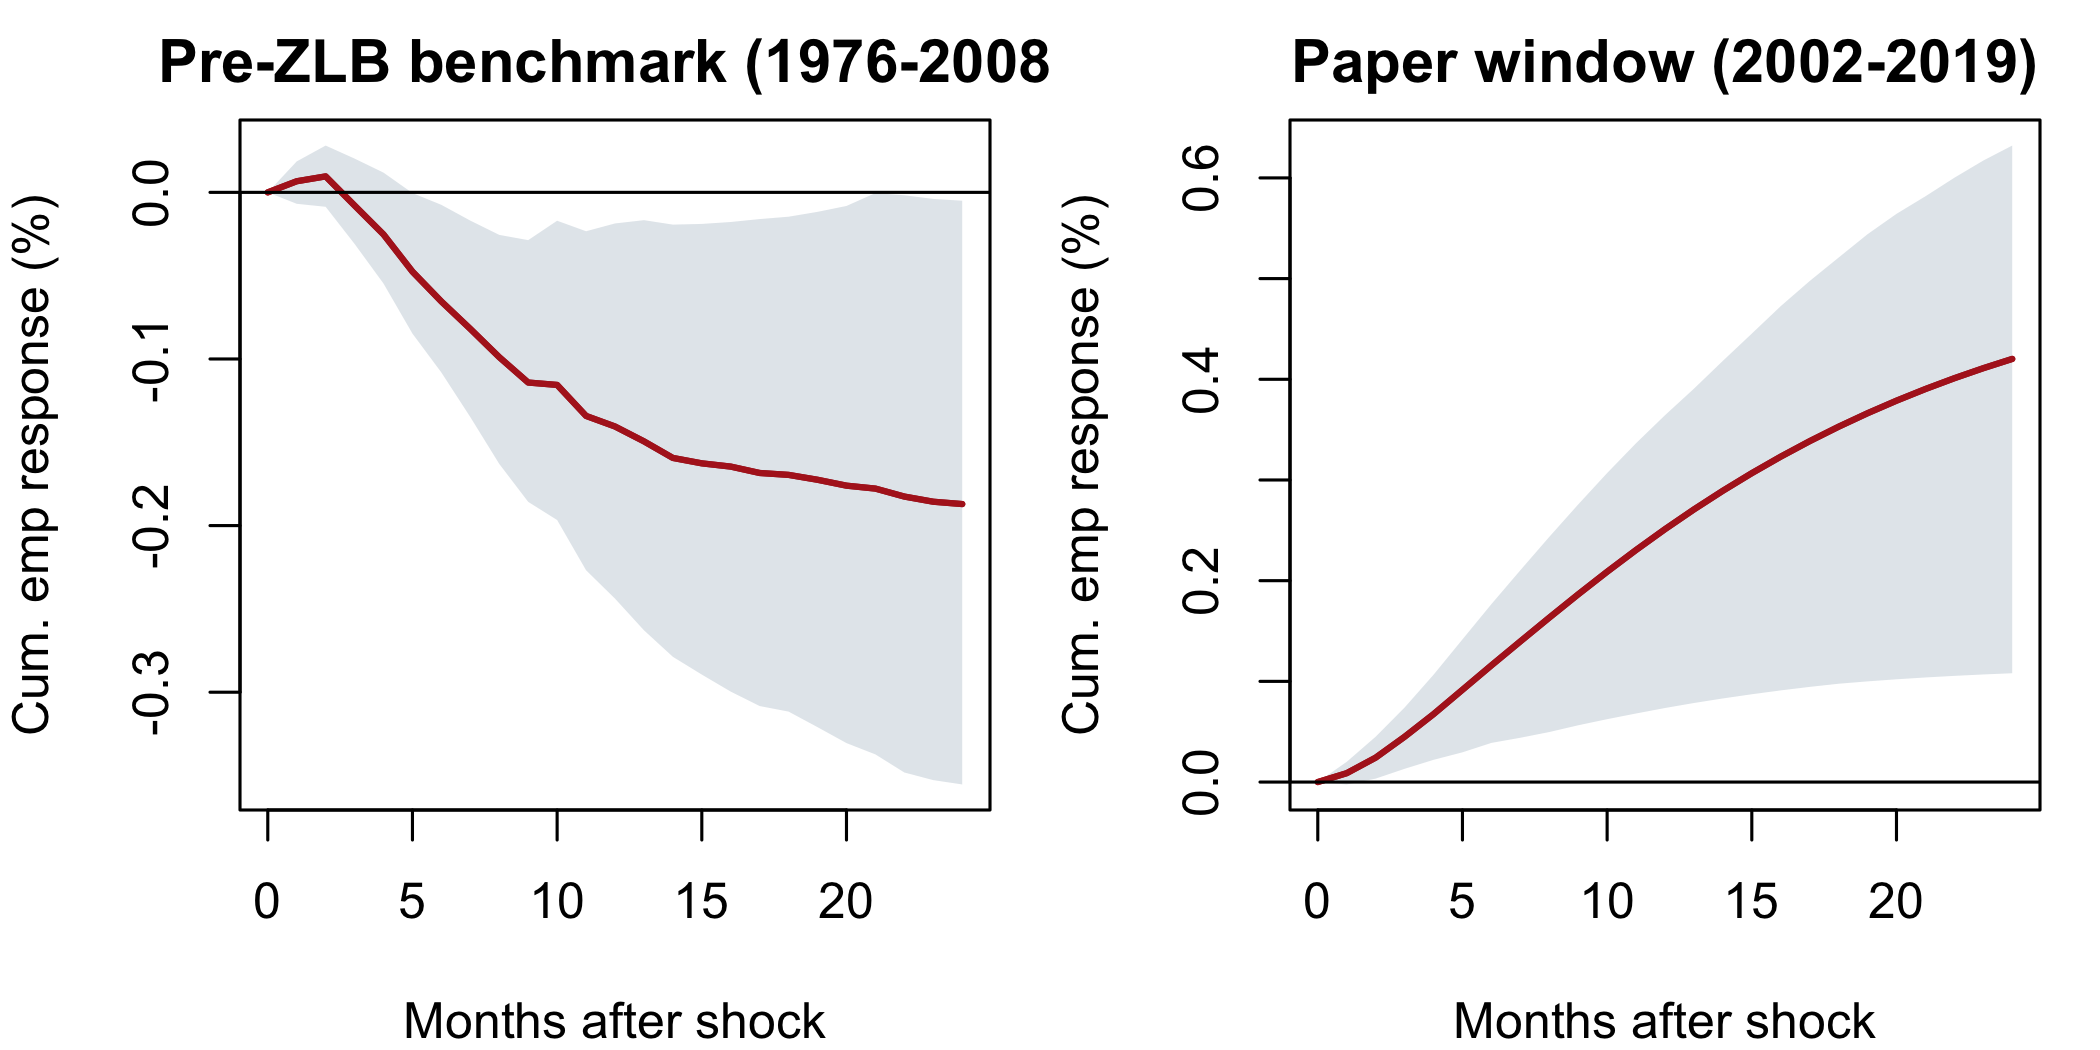
\includegraphics[width=0.86\textwidth]{fig2_var_irf.png}
\caption{Cumulative employment response to a contractionary monetary shock. Left: pre-ZLB
benchmark (1976--2008), the textbook negative response. Right: the 2002--2019 window, where the
ZLB inverts the sign. Shaded bands are 95\% bootstrap intervals.}
\label{fig:varirf}
\end{figure}

\subsection{Structural VAR}
With the recursive ordering $(\pi,n,\Delta r)$ and the monetary shock identified as the funds-rate
innovation, the structural impulse responses (Figure~\ref{fig:svarirf}) confirm the benchmark:
employment falls in a hump-shaped path, troughing near $-0.20\%$ (cumulative $-0.14\%$ at one
year), inflation responds slowly, and the policy rate mean-reverts. The structural and reduced-
form responses coincide in sign and shape, as expected when the only identifying content is the
recursive timing restriction; the SVAR's value added is the explicit economic interpretation of
$\varepsilon^{\text{MP}}$ as an exogenous policy surprise.

\begin{figure}[H]\centering
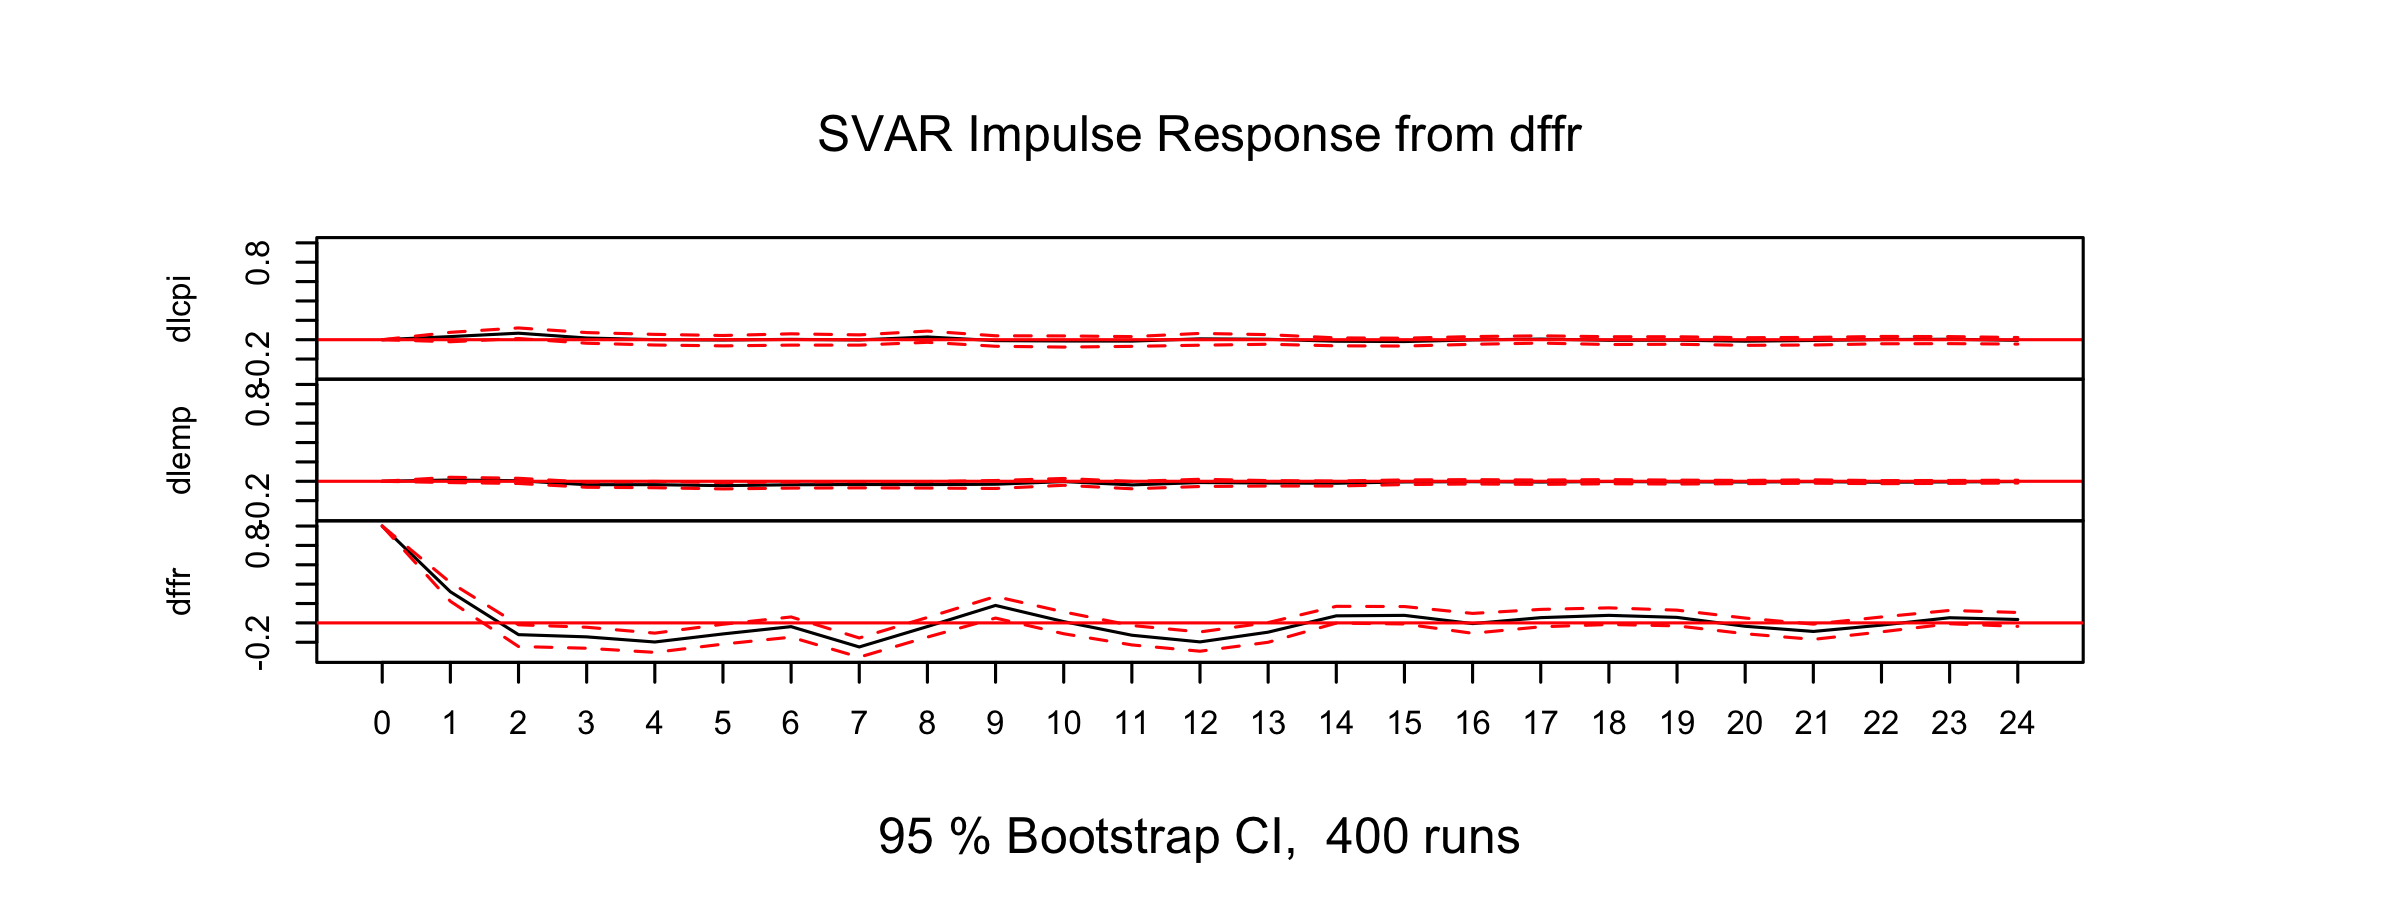
\includegraphics[width=0.92\textwidth]{fig3_svar_irf.png}
\caption{SVAR structural impulse responses to a one-standard-deviation contractionary monetary
shock (recursive identification, 1976--2008). Employment (center) declines in a hump-shaped path.
Shaded bands are 95\% Monte Carlo intervals.}
\label{fig:svarirf}
\end{figure}

\subsection{Local projections: the sign reversal}
Figure~\ref{fig:signflip} and Table~\ref{tab:signflip} present the paper's central result. Using
the \emph{endogenous} funds-rate change in the shift-share interaction (Eq.~\ref{eq:lpint})
reproduces the DiD puzzle: the exposure interaction is positive and strongly significant at every
horizon ($+0.20$ at $h{=}0$ rising to $+1.25$ at $h{=}6$, $t$ up to $6.9$). Replacing it with the
identified Bauer--Swanson surprise \emph{flips the coefficient negative at all horizons}
($-0.39$ to $-2.42$), deepening with horizon: the point estimates are negative at every horizon,
consistent with theory, though imprecisely estimated. The surprise-based estimates are not
individually significant ($|t|\le1.2$), reflecting the limited variation in 72 quarterly shocks;
the contribution is the \emph{contrast}: the precisely estimated positive coefficient is
consistent with an endogeneity artifact, while the identified estimate points negative.

\begin{table}[H]\centering
\caption{Full-panel exposure interaction $\theta_h$: endogenous rate vs.\ identified surprise}
\label{tab:signflip}\small
\begin{tabular}{lcccccc}
\toprule
Horizon $h$ (qtrs) & 0 & 1 & 2 & 4 & 6 & 8 \\
\midrule
$\Delta$FFR $\times$ exp.\ (endogenous) & $0.20^{**}$ & $0.45^{***}$ & $0.73^{***}$ & $1.07^{***}$ & $1.25^{***}$ & $1.16^{***}$ \\
\quad (s.e.) & (.08) & (.10) & (.14) & (.21) & (.26) & (.32) \\
surprise $\times$ exp.\ (identified) & $-0.39$ & $-0.73$ & $-1.17$ & $-1.62$ & $-1.92$ & $-2.01$ \\
\quad (s.e.) & (.50) & (.71) & (.99) & (1.85) & (2.63) & (2.96) \\
\bottomrule
\end{tabular}
\\[2pt]
\footnotesize Outcome: $100(\ell_{i,t+h}-\ell_{i,t-1})$. County + time FE; SE clustered by
quarter. Exposure standardized. $^{*}p<.10$, $^{**}p<.05$, $^{***}p<.01$.
\end{table}

\begin{figure}[H]\centering
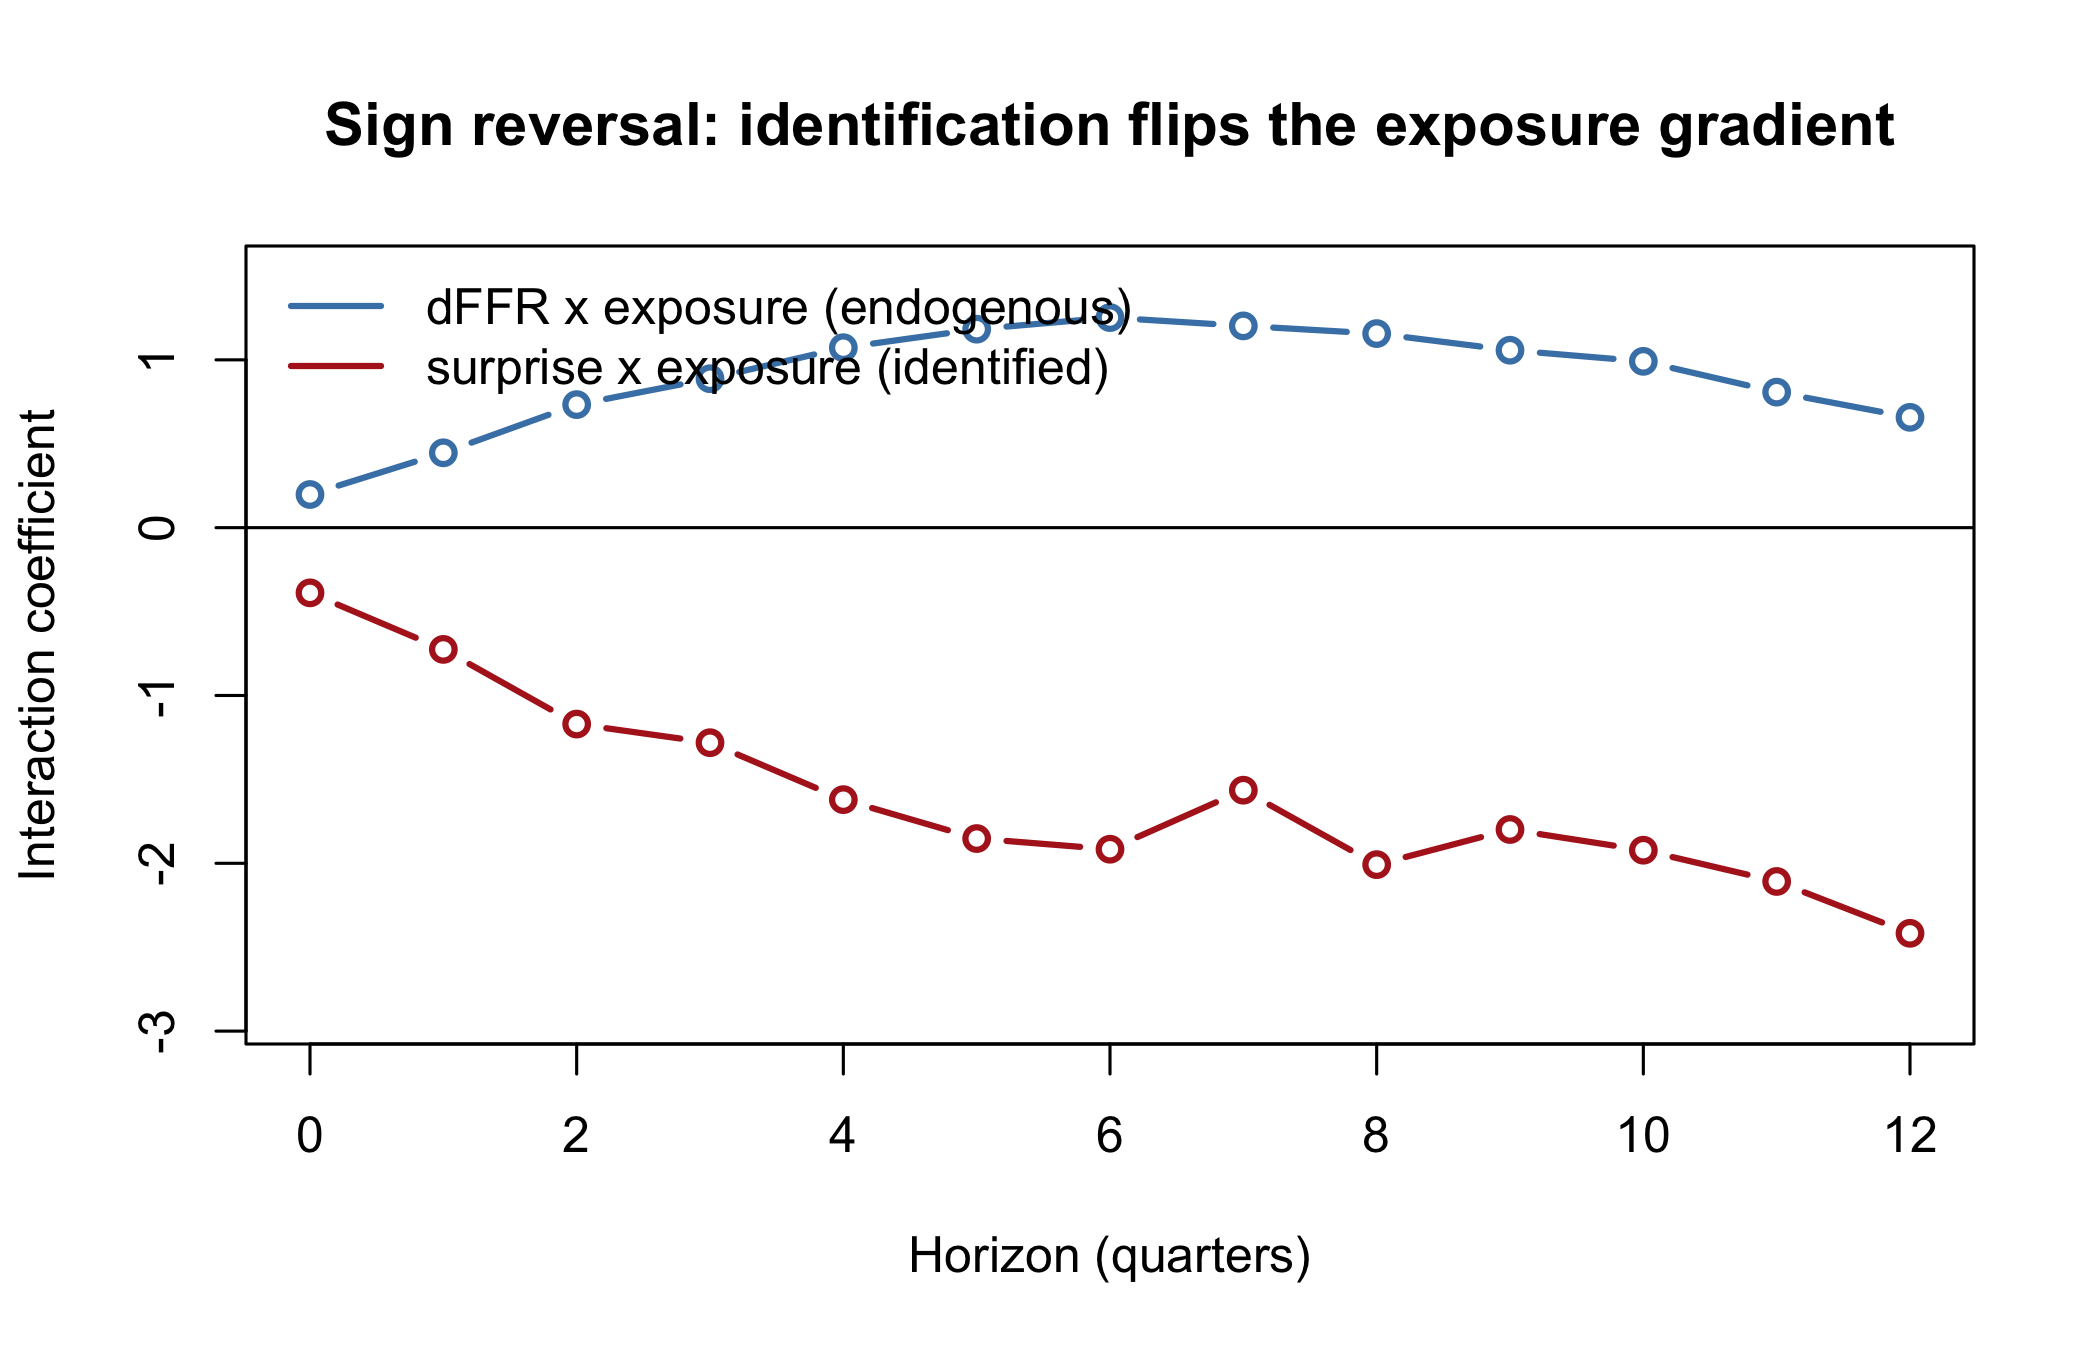
\includegraphics[width=0.78\textwidth]{fig4_signflip.png}
\caption{The sign reversal. Holding the shift-share design fixed and swapping only the source of
policy variation flips the exposure interaction from significantly positive (endogenous
$\Delta$FFR) to negative (identified surprise). Bands are 95\% (quarter-clustered).}
\label{fig:signflip}
\end{figure}

The focused panel of five major counties (Los Angeles, Cook/Chicago, New York, Harris/Houston,
Maricopa/Phoenix), following the proposal feedback to narrow the LP, gives a consistent dynamic
picture: the pooled employment response to an identified tightening surprise is negative and
deepening to roughly $-8\%$ over three years (Figure~\ref{fig:lpbig}), again imprecise.
Reassuringly, the LP and VAR employment responses share the same hump-shaped contraction once
placed on a common scale (Figure~\ref{fig:lpvar}); since \citet{plagborg2021} prove LP and VAR
target the same population responses, this agreement is expected, with cross-method differences
reflecting shock measurement rather than the estimator \citep{coibion2012}.

\begin{figure}[H]\centering
\begin{minipage}[t]{0.49\textwidth}\centering
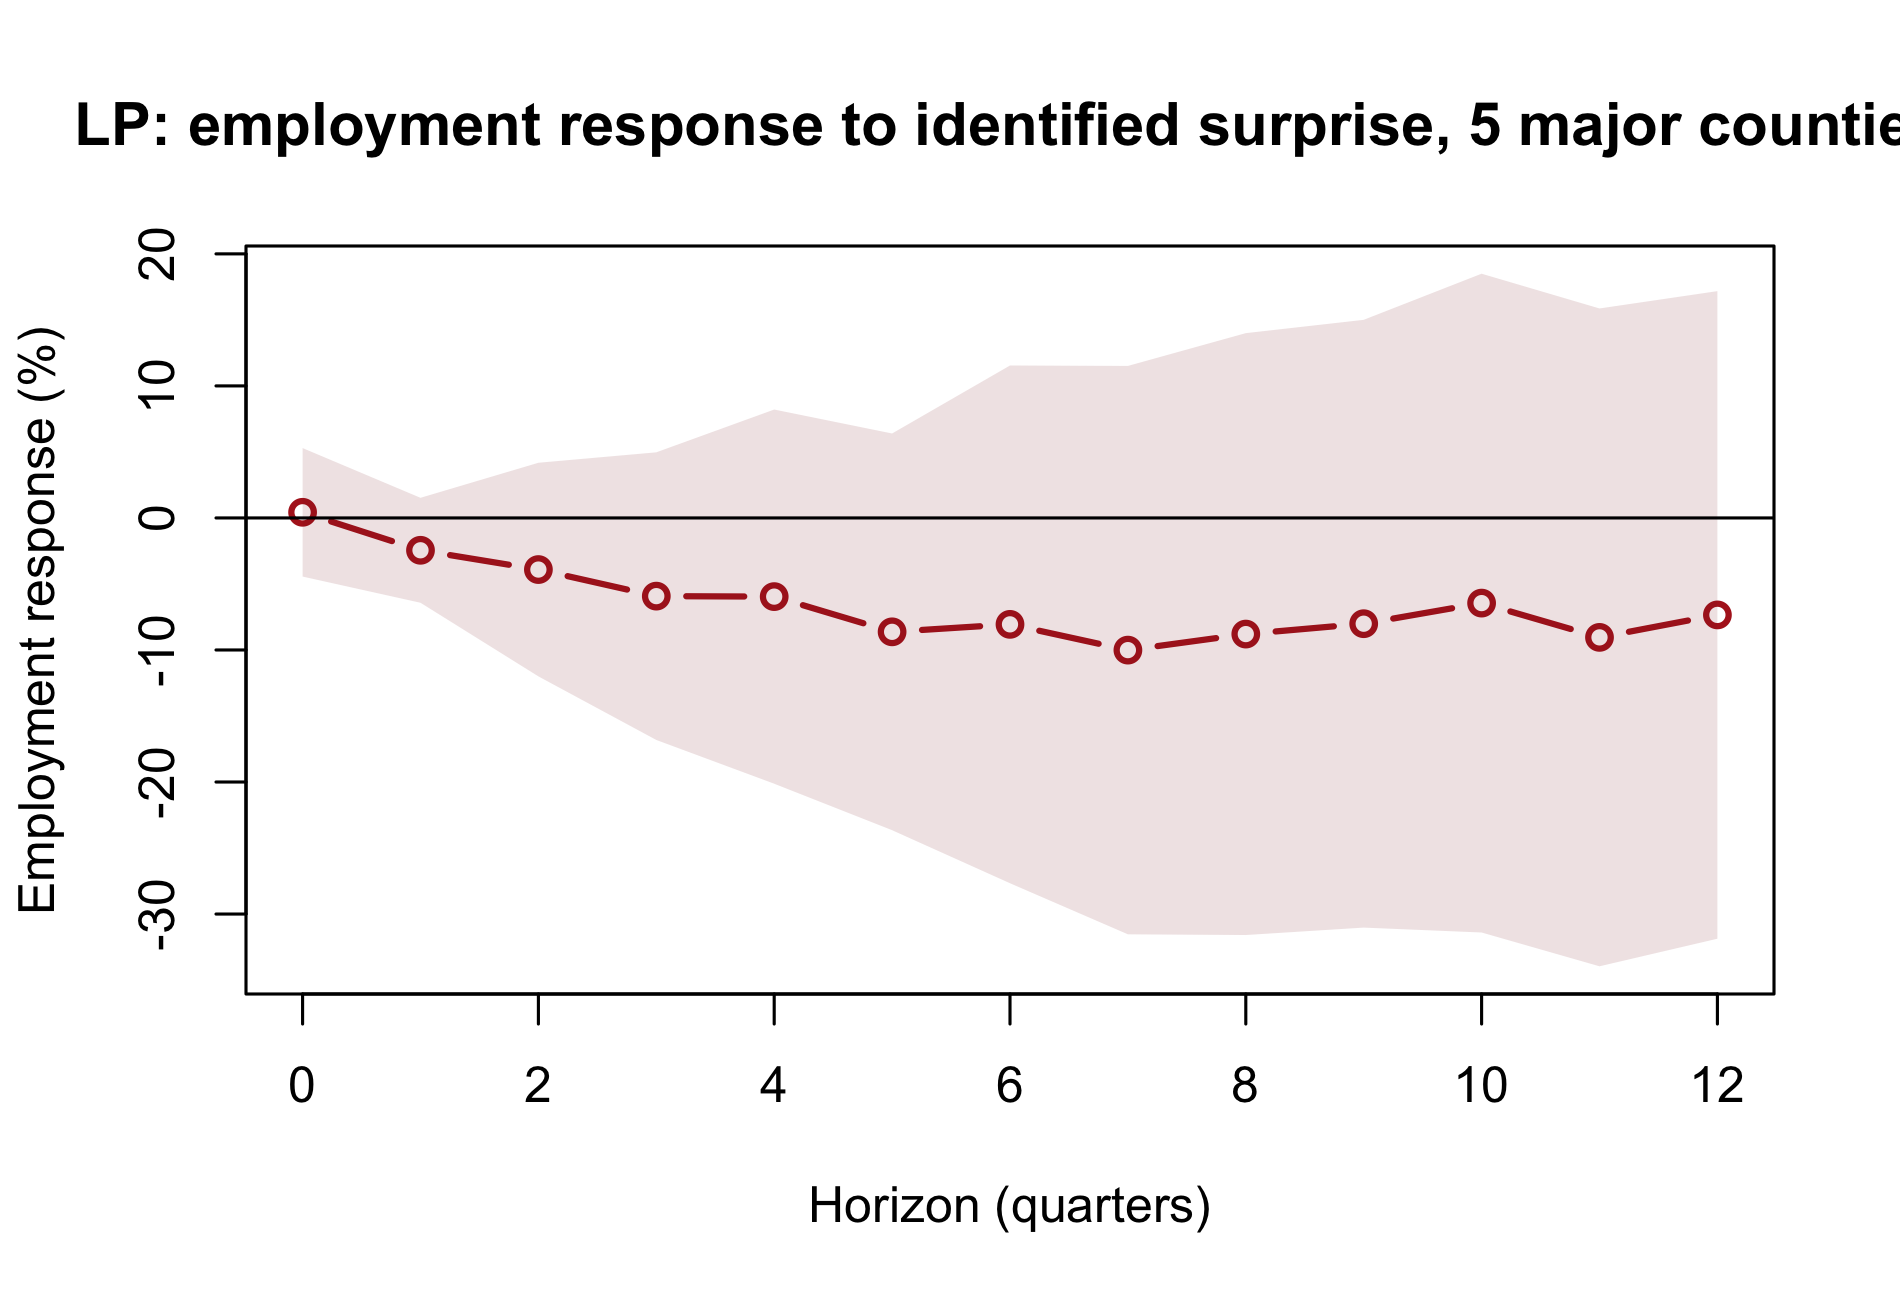
\includegraphics[width=\textwidth]{fig5_lp_bigcounty.png}
\caption{LP: employment response to an identified surprise, five major counties.}
\label{fig:lpbig}
\end{minipage}\hfill
\begin{minipage}[t]{0.49\textwidth}\centering
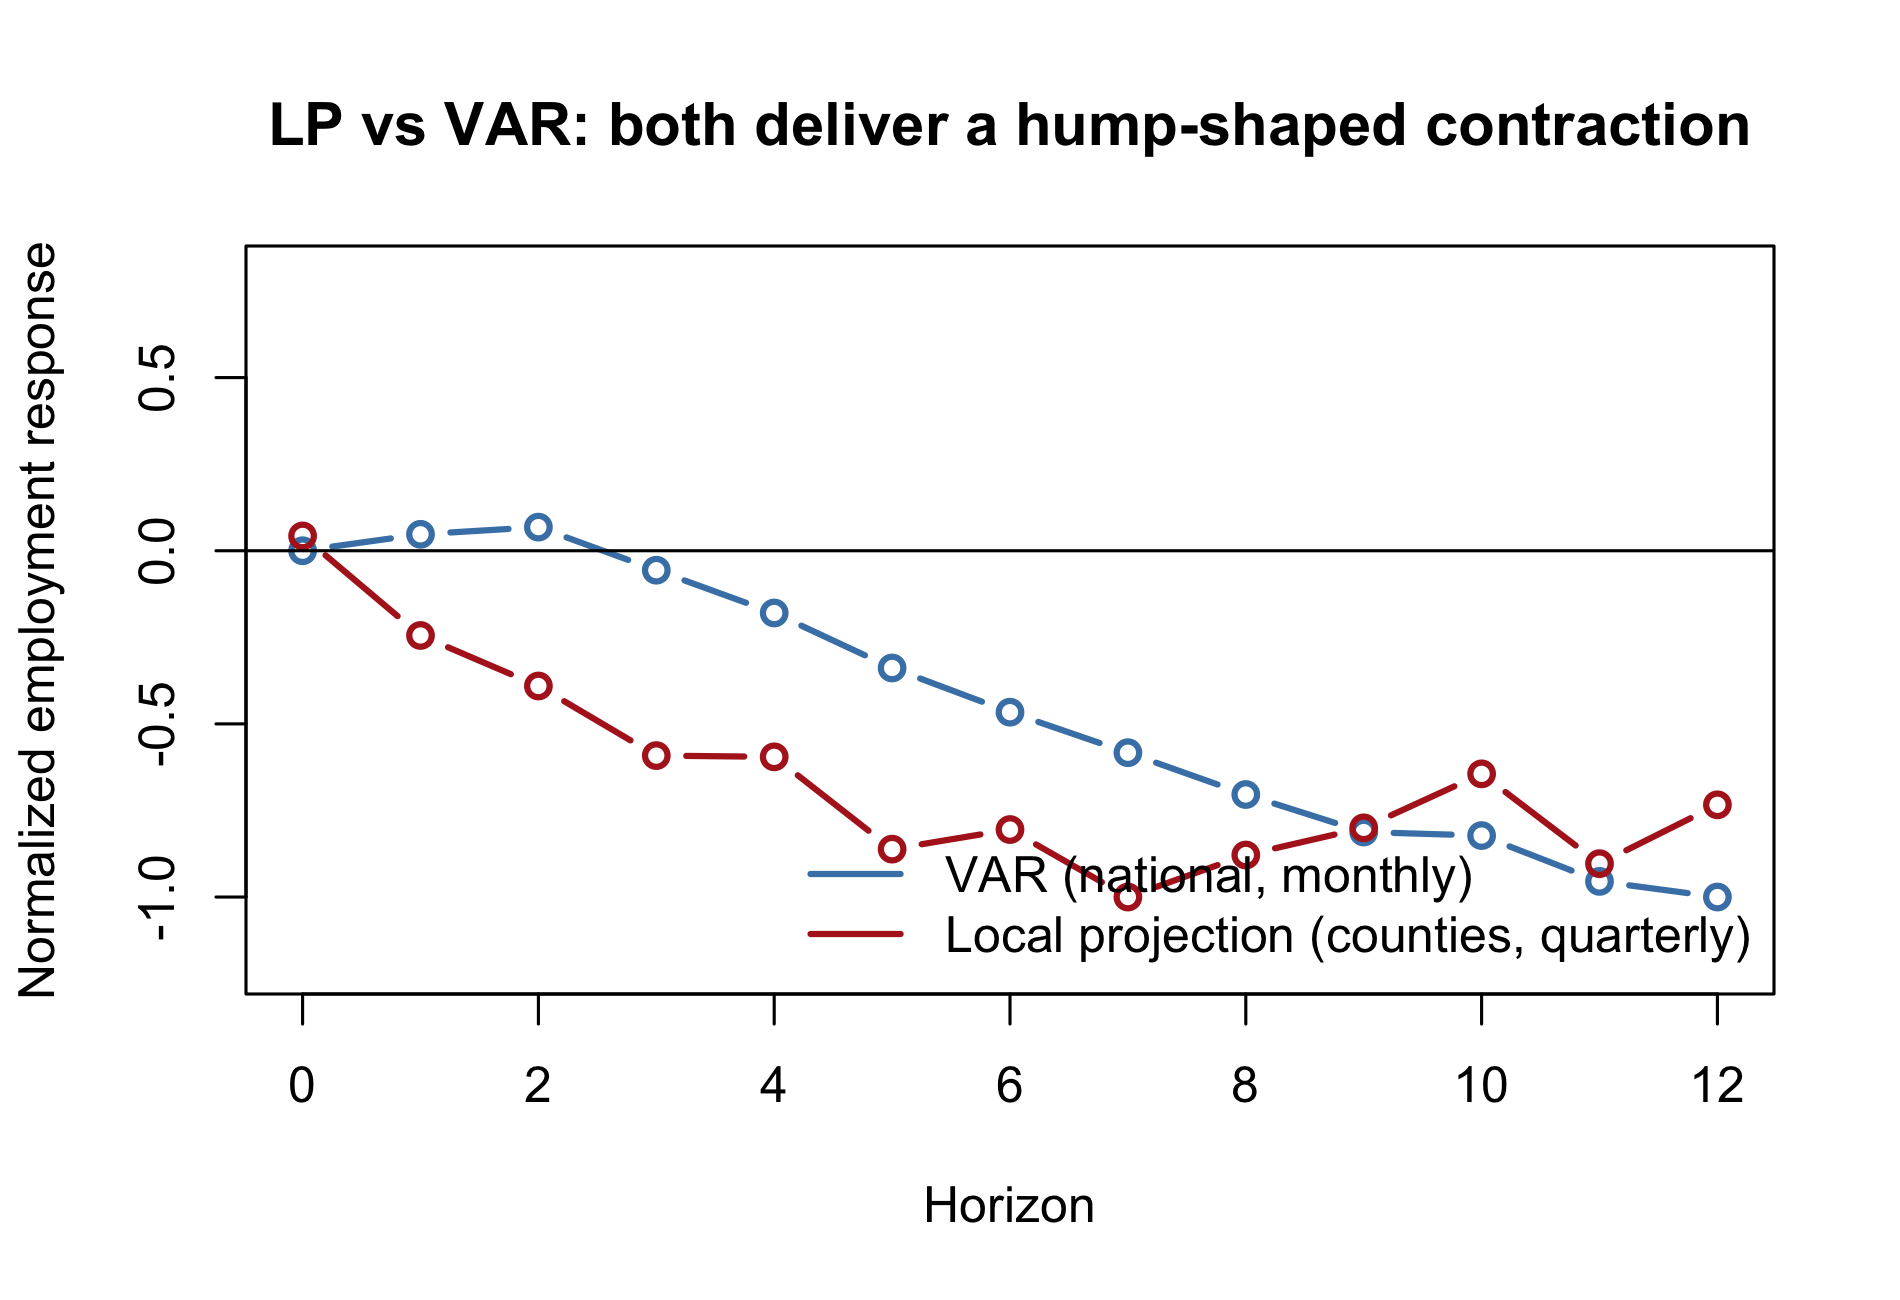
\includegraphics[width=\textwidth]{fig6_lp_vs_var.png}
\caption{LP vs.\ VAR employment responses (normalized): both hump-shaped contractions.}
\label{fig:lpvar}
\end{minipage}
\end{figure}

\emph{A caution on the cross-section.} The exposure gradient is not robust to county size.
Among the 20 largest counties split by exposure (so size is held roughly fixed), high- and
low-exposure metros contract \emph{similarly} after an identified shock (difference $|t|<1.3$
at all horizons): extreme-exposure counties are small, specialized places, so a na\"ive high-vs-
low split confounds exposure with size and diversification. The honest reading---reinforcing the
thesis---is that \emph{identification}, not a cross-sectional exposure channel, drives the sign:
clean shocks lower employment broadly, and the DiD's positive interaction was an endogeneity
artifact.

\subsection{Random forest}
Out-of-sample, the random forest attains a lower average RMSE ($0.059$) than the random-walk
($0.081$) and seasonal-naive ($0.084$) benchmarks across rolling test years
(Table~\ref{tab:rfcv}). But this is not forecasting skill: the correlation between RF forecasts
and realized employment growth is $-0.03$, and over the 2014--2019 expansion the RF essentially
predicts the stable positive mean (Figure~\ref{fig:rf}, right). The RMSE ``win'' is variance
shrinkage toward the conditional mean in a low-volatility expansion, not genuine predictability;
directional accuracy is trivially high only because growth was positive in every test month.
Variable importance (Figure~\ref{fig:rf}, left) loads almost entirely on own lags of employment
growth, and the partial dependence on the first lag (Figure~\ref{fig:rfpdp}) is nearly flat---
consistent with weak short-horizon predictability of the aggregate. This tempers the optimism of
\citet{medeiros2021}: random forests help for some series and horizons, but here they add no skill
beyond a na\"ive benchmark.

\begin{table}[H]\centering
\caption{Random forest rolling-origin out-of-sample RMSE and MAE}\label{tab:rfcv}\small
\begin{tabular}{lccccc}
\toprule
Test year & RF RMSE & RW RMSE & Seas.-naive RMSE & RF MAE & RW MAE \\
\midrule
2014 & 0.065 & 0.063 & 0.081 & 0.055 & 0.055 \\
2015 & 0.054 & 0.083 & 0.074 & 0.044 & 0.074 \\
2016 & 0.064 & 0.099 & 0.096 & 0.054 & 0.088 \\
2017 & 0.036 & 0.037 & 0.078 & 0.030 & 0.029 \\
2018 & 0.068 & 0.100 & 0.066 & 0.055 & 0.090 \\
2019 & 0.066 & 0.103 & 0.108 & 0.055 & 0.091 \\
\midrule
Mean & \textbf{0.059} & 0.081 & 0.084 & \textbf{0.049} & 0.071 \\
\bottomrule
\end{tabular}
\\[2pt]
\footnotesize Despite the RMSE/MAE edge, corr(forecast, actual) $=-0.03$: variance shrinkage, not skill.
\end{table}

\begin{figure}[H]\centering
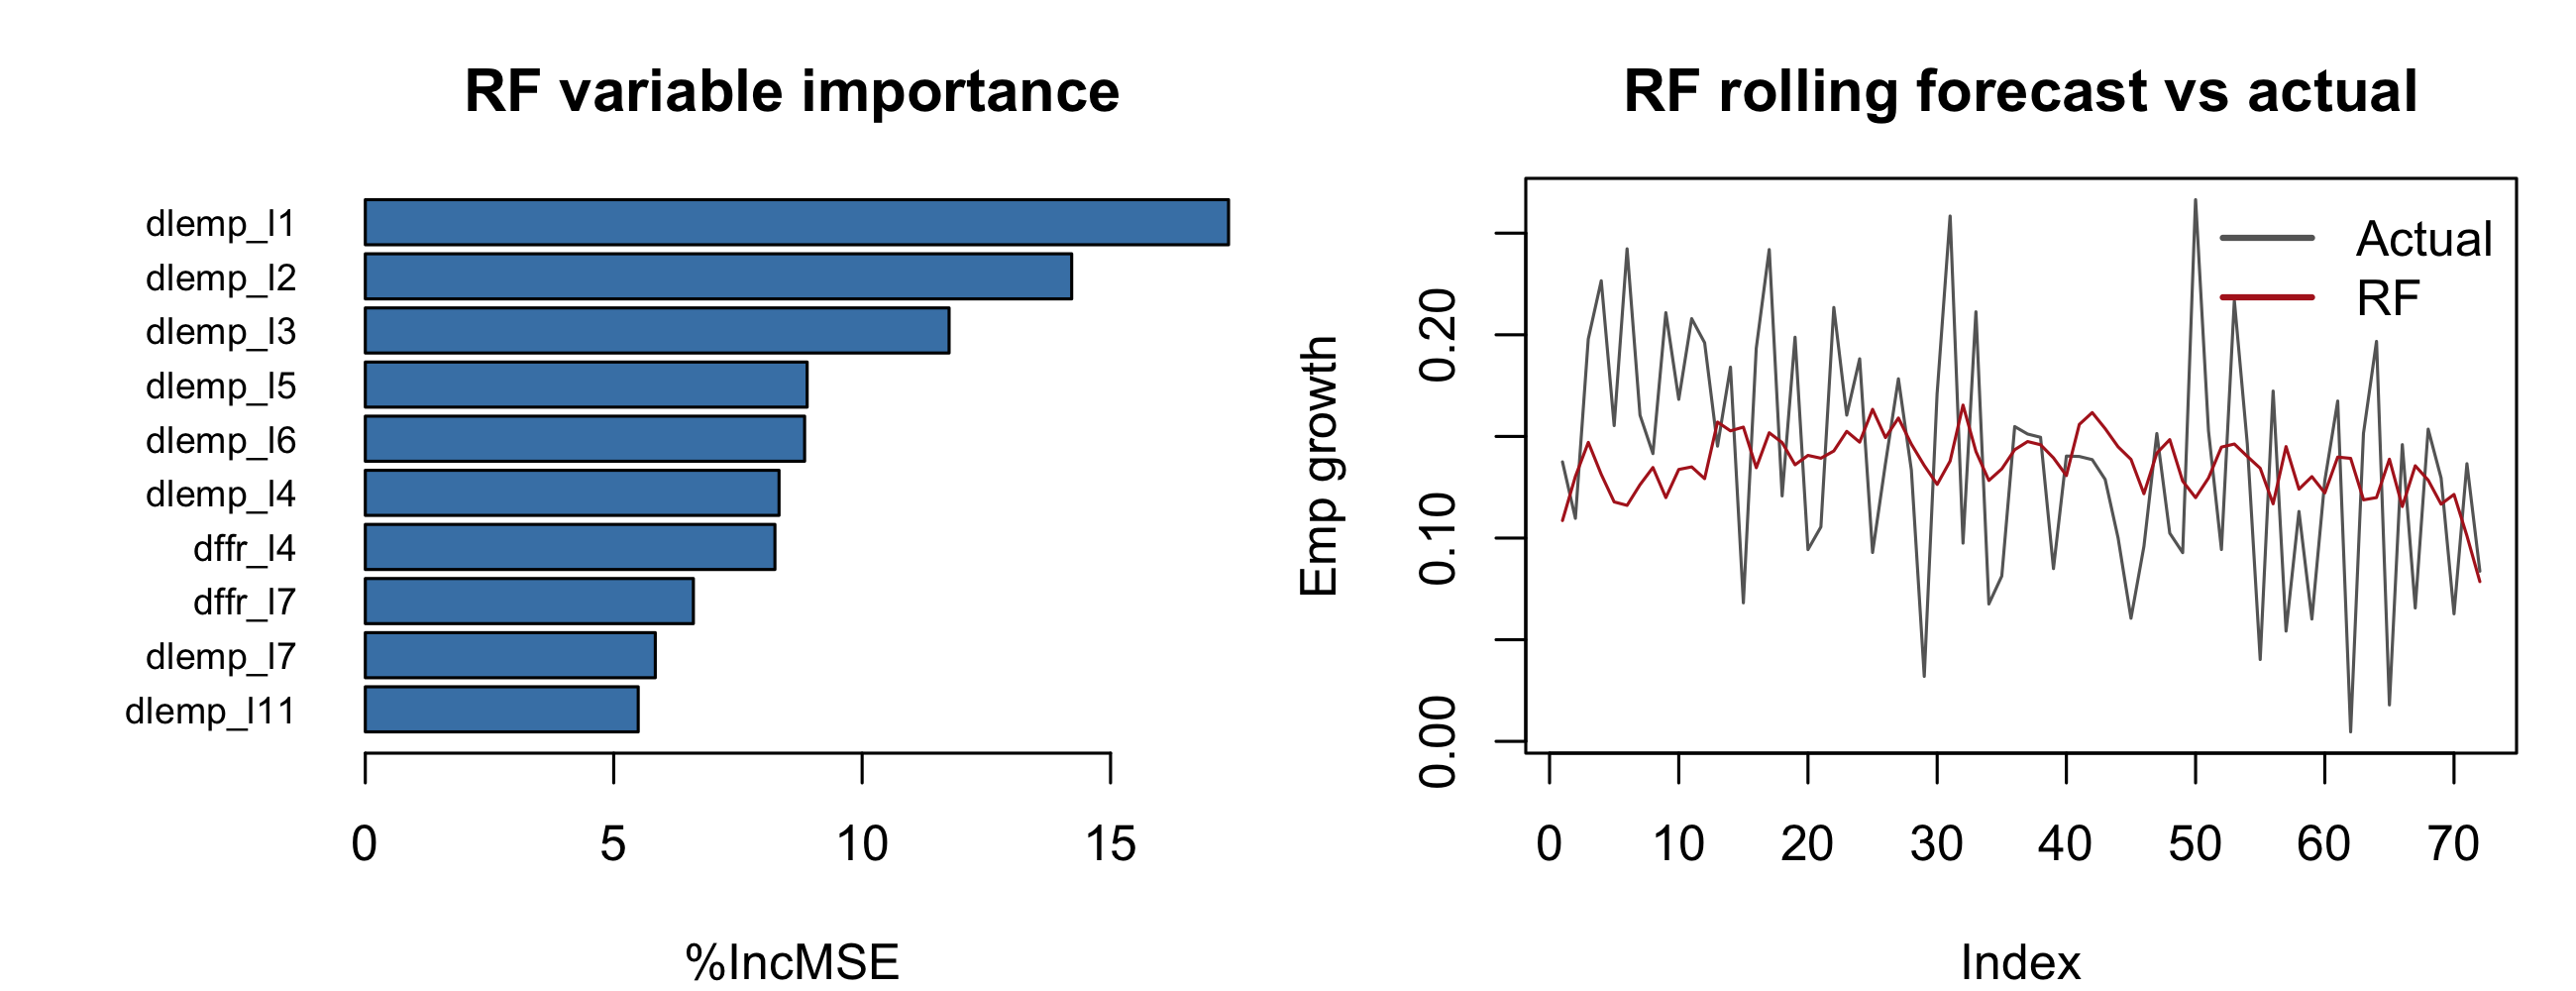
\includegraphics[width=0.96\textwidth]{fig7_rf.png}
\caption{Random forest. Left: variable importance loads on own employment-growth lags. Right:
rolling forecasts track the expansion mean but not the fluctuations (corr $=-0.03$).}
\label{fig:rf}
\end{figure}

\begin{figure}[H]\centering
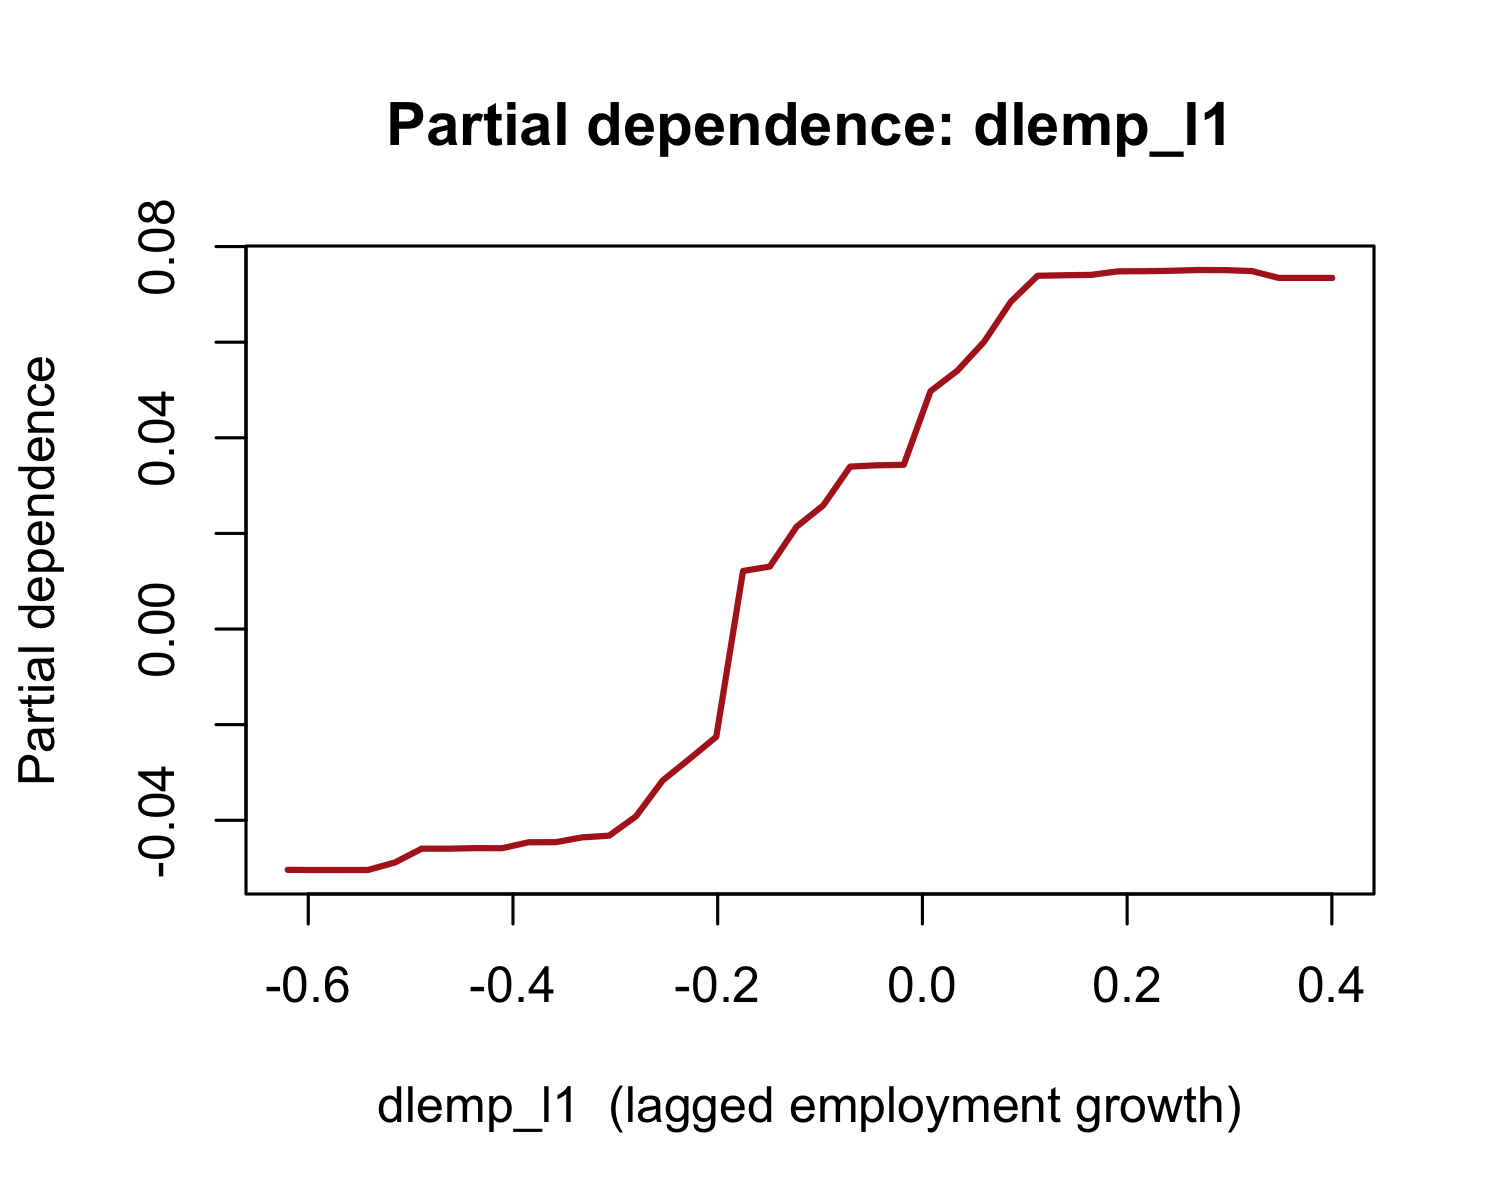
\includegraphics[width=0.52\textwidth]{fig8_rf_pdp.png}
\caption{Partial dependence of forecast employment growth on its first lag---nearly flat.}
\label{fig:rfpdp}
\end{figure}

\section{Conclusion}

This paper adjudicated between two explanations for a counterintuitive positive employment
response to monetary tightening in a county shift-share design. The evidence points to
\textbf{identification, not aggregation}. Reduced-form and structural VARs reproduce the textbook
contractionary employment response on a clean pre-ZLB sample, and the same VAR inverts over
2002--2019 only because the zero lower bound strips the funds rate of policy content. Most
directly, holding the shift-share design fixed and replacing the endogenous funds-rate change
with an identified Bauer--Swanson surprise flips the exposure interaction from significantly
positive to negative at every horizon. The most plausible reading is that the positive sign is an
endogeneity artifact and the underlying effect is contractionary---though, given the imprecision of
the surprise-based estimates, this is strongly suggestive rather than definitively established.

Relative to \citet{carlino1998} and the identification literature \citep{cee1999,coibion2012},
the paper's contribution is to show concretely how endogeneity can manufacture a sign reversal
inside an otherwise standard regional design, and how a high-frequency external shock
\citep{bauerswanson2023} restores the expected contractionary sign. The finding is therefore as
much methodological as substantive: it cautions that shift-share designs built on the realized
policy rate can mislead precisely where the policy rate is most endogenous.

These conclusions come with real limits. The surprise-based estimates are imprecise, because
seventy-two quarters of monetary surprises provide limited identifying variation, so the negative
interaction is directional rather than statistically significant, and an instrumental-variables
projection is infeasible because the orthogonalized surprise does not move the realized quarterly
rate. The cross-sectional exposure gradient, in turn, is confounded with county size and does not
survive once size is held fixed. A deeper alternative I cannot fully rule out is the central-bank
information effect \citep{nakamura2018,jarocinski2020}: if the surprises blend pure policy and
information shocks, part of the interaction may reflect favorable news rather than endogeneity,
and decomposing the two is the priority extension. Other natural steps include a Wu--Xia shadow
rate \citep{wuxia2016} to recover policy content through the zero lower bound, a longer surprise
sample, and Driscoll--Kraay or wild-cluster inference to sharpen the panel projection. The
random-forest exercise, meanwhile, stands as its own cautionary note: a lower RMSE need not mean
genuine predictive skill.

\clearpage
\renewcommand{\refname}{Bibliography}
\begin{thebibliography}{99}
\bibitem[Bauer and Swanson(2023)]{bauerswanson2023} Bauer, Michael D., and Eric T. Swanson. 2023. ``A Reassessment of Monetary Policy Surprises and High-Frequency Identification.'' \textit{NBER Macroeconomics Annual} 37: 87--155.
\bibitem[Borusyak et al.(2022)]{borusyak2022} Borusyak, Kirill, Peter Hull, and Xavier Jaravel. 2022. ``Quasi-Experimental Shift-Share Research Designs.'' \textit{Review of Economic Studies} 89(1): 181--213.
\bibitem[Carlino and DeFina(1998)]{carlino1998} Carlino, Gerald, and Robert DeFina. 1998. ``The Differential Regional Effects of Monetary Policy.'' \textit{Review of Economics and Statistics} 80(4): 572--587.
\bibitem[Christiano et al.(1999)]{cee1999} Christiano, Lawrence J., Martin Eichenbaum, and Charles L. Evans. 1999. ``Monetary Policy Shocks: What Have We Learned and to What End?'' In \textit{Handbook of Macroeconomics}, vol.\ 1A, ed.\ J.B. Taylor and M. Woodford, 65--148. Amsterdam: Elsevier.
\bibitem[Coibion(2012)]{coibion2012} Coibion, Olivier. 2012. ``Are the Effects of Monetary Policy Shocks Big or Small?'' \textit{American Economic Journal: Macroeconomics} 4(2): 1--32.
\bibitem[Gertler and Karadi(2015)]{gertlerkaradi2015} Gertler, Mark, and Peter Karadi. 2015. ``Monetary Policy Surprises, Credit Costs, and Economic Activity.'' \textit{American Economic Journal: Macroeconomics} 7(1): 44--76.
\bibitem[Goldsmith-Pinkham et al.(2020)]{gpss2020} Goldsmith-Pinkham, Paul, Isaac Sorkin, and Henry Swift. 2020. ``Bartik Instruments: What, When, Why, and How.'' \textit{American Economic Review} 110(8): 2586--2624.
\bibitem[G\"urkaynak et al.(2005)]{gss2005} G\"urkaynak, Refet S., Brian Sack, and Eric T. Swanson. 2005. ``Do Actions Speak Louder Than Words? The Response of Asset Prices to Monetary Policy Actions and Statements.'' \textit{International Journal of Central Banking} 1(1): 55--93.
\bibitem[Jaroci\'nski and Karadi(2020)]{jarocinski2020} Jaroci\'nski, Marek, and Peter Karadi. 2020. ``Deconstructing Monetary Policy Surprises: The Role of Information Shocks.'' \textit{American Economic Journal: Macroeconomics} 12(2): 1--43.
\bibitem[Jord\`a(2005)]{jorda2005} Jord\`a, \`Oscar. 2005. ``Estimation and Inference of Impulse Responses by Local Projections.'' \textit{American Economic Review} 95(1): 161--182.
\bibitem[Medeiros et al.(2021)]{medeiros2021} Medeiros, Marcelo C., Gabriel F.R. Vasconcelos, \`Alvaro Veiga, and Eduardo Zilberman. 2021. ``Forecasting Inflation in a Data-Rich Environment: The Benefits of Machine Learning Methods.'' \textit{Journal of Business \& Economic Statistics} 39(1): 98--119.
\bibitem[Nakamura and Steinsson(2018)]{nakamura2018} Nakamura, Emi, and J\'on Steinsson. 2018. ``High-Frequency Identification of Monetary Non-Neutrality: The Information Effect.'' \textit{Quarterly Journal of Economics} 133(3): 1283--1330.
\bibitem[Plagborg-M\o ller and Wolf(2021)]{plagborg2021} Plagborg-M\o ller, Mikkel, and Christian K. Wolf. 2021. ``Local Projections and VARs Estimate the Same Impulse Responses.'' \textit{Econometrica} 89(2): 955--980.
\bibitem[Stock and Watson(2018)]{stockwatson2018} Stock, James H., and Mark W. Watson. 2018. ``Identification and Estimation of Dynamic Causal Effects in Macroeconomics Using External Instruments.'' \textit{The Economic Journal} 128(610): 917--948.
\bibitem[Wu and Xia(2016)]{wuxia2016} Wu, Jing Cynthia, and Fan Dora Xia. 2016. ``Measuring the Macroeconomic Impact of Monetary Policy at the Zero Lower Bound.'' \textit{Journal of Money, Credit and Banking} 48(2--3): 253--291.
\end{thebibliography}

\appendix
\section{Appendix: R Code}
The complete, commented R script reproducing every table and figure is submitted separately as
\texttt{Dalis\_Abdallah\_ECO508\_Code.R.txt}. It loads the QCEW county panel and CBP exposure
shares, downloads the FRED series and the Bauer--Swanson surprises, and runs the VAR, SVAR,
local projections, and random forest end-to-end.

\end{document}
